\chapter{Preparation for H(Inv) decays in the VBF channel with CMS parked data}
\label{CHAPTER:PreparationParkedDataAnalysis}

%%%%%%%%%%%%%%%%%%%%%%%%%%%%%%%%%%%%%%%%%%%%%%%%%%%%%%%%%%%%%%%%%%%%%%%%%%%%%%%%%%%%
%%% SECTION
%%%%%%%%%%%%%%%%%%%%%%%%%%%%%%%%%%%%%%%%%%%%%%%%%%%%%%%%%%%%%%%%%%%%%%%%%%%%%%%%%%%%
\section{QCD VBF+MET Monte Carlo simulation}

\begin{table}
\centering
\begin{tabular}{|c|r|c|r|c|c|}
  \hline
  Sample          &       Ev. Gen. & Filter Eff. &  Events &  XS $[pb]$ & Eq. Lumi. $[fb^{-1}]$ \\
  \hline \hline
  QCD-Pt-80to120  & 39376000000 &    0.000049 & 1614416 &  1033680 &  38.09 \\
  QCD-Pt-120to170 &  7000000000 &    0.000283 & 2051000 & 156293.3 &  44.79 \\
  QCD-Pt-170to300 &  1375000000 &    0.000987 & 1391500 & 34138.15 &  40.28 \\
  QCD-Pt-300to470 &    80000000 &    0.002659 &  207840 & 1759.549 &  45.47 \\
  QCD-Pt-470to600 &    25000000 &    0.004127 &  104675 & 113.8791 & 219.53 \\
  \hline
\end{tabular}
\end{table}

\begin{figure}[h!]
\centering
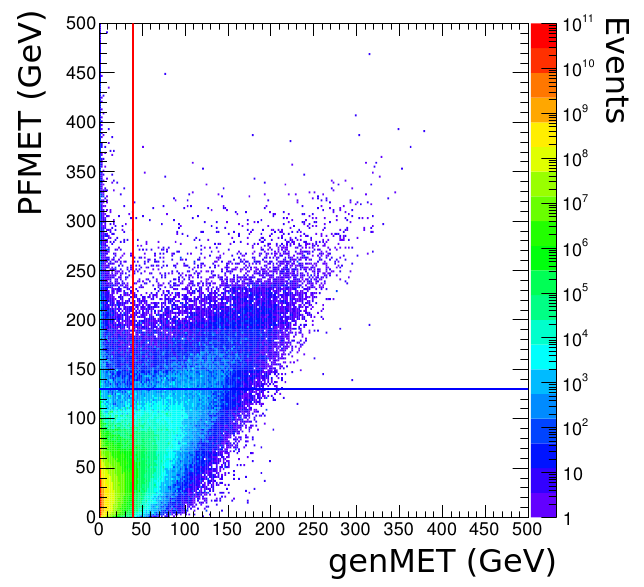
\includegraphics[width=0.55\textwidth]{Chapter05/ParkedDataPreparation/Images/Joao_140209_p11.png}
\caption{Reconstructed PFMET as a function of generator-level MET
      in the inclusive QCD samples $80 < \hat{p_T} < 600$ GeV before
      any selection.}
\label{fig:qcdRecovsGenMET}
\end{figure}

\section{Dijet-MET system topological variables}


\section{Track distribution variables}


% %%%%%%%%%%%%%%%%%%%%%%%%%%%%%%%%%%%%%%%%%%%%%%%%%%%%%%%%%%
% Jet topology variables
% %%%%%%%%%%%%%%%%%%%%%%%%%%%%%%%%%%%%%%%%%%%%%%%%%%%%%%%%%%
% 18 Months report was on the Sep 9 2013
% 
% /home/hep/jca10/work/vbfinv/ws04/CMSSW_5_3_11/src/UserCode/ICHiggsTauTau/Analysis/HiggsNuNu/PLOTS_mjj1200_dijetFrac/nunu/MET130/n_vtx_2012_DijetFraction_log.pdf
% Looks like plots are from Jun 25 2013
% 
% FOUND FILE: This is the file used in the plots for the 18 months report
% /home/hep/jca10/work/vbfinv/ws04/CMSSW_5_3_11/src/UserCode/ICHiggsTauTau/Analysis/HiggsNuNu/output_mjj1100_dijetFrac/nunu/MET130/MC_VBF_HToZZTo4Nu_M-120.root
% 
% /vols/cms02/jca10/work/ws01/CMSSW_5_3_11/src/UserCode/ICHiggsTauTau/Analysis/HiggsNuNu/plots/DPhiSIGNAL_CJVpass/dijetMet/dijetFrac_htMET.png
% Looks like plots are from Feb 20 2014


% %%%%%%%%%%%%%%%%%%%%%%%%%%%%%%%%%%%%%%%%%%%%%%%%%%%%%%%%%%
% Track variables
% %%%%%%%%%%%%%%%%%%%%%%%%%%%%%%%%%%%%%%%%%%%%%%%%%%%%%%%%%%
% 20140603_ICVBFHiggs_JPela.pdf
% /afs/cern.ch/user/p/pela/work/cms/vbfinv/ws03/CMSSW_5_3_11/src/VBFHiggsToInvisible/VariableAnalyser/python/PowhegSignal_cfi.py
% 
% %%%%%%%%%%%%%%%%%%%%%%%%%%%%%%%%%%%%%%%%%%%%%%%%%%%%%%%%%%
% QCD VFB + MET samples
% %%%%%%%%%%%%%%%%%%%%%%%%%%%%%%%%%%%%%%%%%%%%%%%%%%%%%%%%%%
% 20140204_ICVBFHiggs_JPela_VBFQCD.pdf (plot on the AN)
% 20140506_ICVBFHiggs_JPela.pdf (selection test)
% 
% Something odd here
% /home/hep/jca10/work/vbfinv/ws08/CMSSW_5_3_11/src/UserCode/ICHiggsTauTau/Analysis/HiggsNuNu

%%%%%%%%%%%%%%%%%%%%%%%%%%%%%%%%%%%%%%%%%%%%%%%%%%%%%%%%%%%%%%%%%%%%%%%%%%%%%%%%%%%
%%%%%%%%%%%%%%%%%%%%%%%%%%%%%%%%%%%%%%%%%%%%%%%%%%%%%%%%%%%%%%%%%%%%%%%%%%%%%%%%%%%
%%%%%%%%%%%%%%%%%%%%%%%%%%%%%%%%%%%%%%%%%%%%%%%%%%%%%%%%%%%%%%%%%%%%%%%%%%%%%%%%%%%

